\documentclass[times, utf8, zavrsni, numeric]{fer}
\usepackage{booktabs}
\usepackage{longtable}
\usepackage{float}
\usepackage{url}
\usepackage{listings}
\lstset{language=bash}

\begin{document}

% \renewcommand*\contentsname{Table of contents}

% TODO: Navedite broj rada.
\thesisnumber{6902}

% TODO: Navedite naslov rada.
\title{Pipeline for Detection Clusters of Modified Nucleotides in Nanopore Sequenced RNA Reads}

% TODO: Navedite vaše ime i prezime.
\author{Ivona Martinović}

\maketitle

% Ispis stranice s napomenom o umetanju izvornika rada. Uklonite naredbu \izvornik ako želite izbaciti tu stranicu.
\izvornik

% Ispis stranice s napomenom o umetanju izvornika rada. Uklonite naredbu \izvornik ako želite izbaciti tu stranicu.
\izvornik

% Dodavanje zahvale ili prazne stranice. Ako ne želite dodati zahvalu, naredbu ostavite radi prazne stranice.
\zahvala{
I am profoundly grateful to my mentor, Professor Mile Šikić and teaching assistants 
Robert Vaser and Josip Marić for their guidance, patience, time and sharing their 
knowledge with me.
}

\tableofcontents

\chapter{Introduction}
Although RNA is a single-stranded molecule, researchers have discovered that 
it can form double-stranded structures. Also, single-stranded RNA can form many 
secondary structures in which a single RNA molecule folds over and forms hairpin 
loops. Such base-pairing of RNA is critical for many RNA functions. 
One of the approaches for quantification of specific structures of RNA molecules 
is the modification of exposed nucleotides. The modification is done artificially 
in a laboratory. After unfolding such RNA by looking at its primary sequence, one 
observes characteristic patterns of positions of modified nucleotides for each 
cluster of structures \cite{RNAstructure}.

Third-generation sequencing technologies, such as Oxford Nanopore Technologies, 
facilitated the analysis of RNA due to their ability to read considerably longer 
fragments than their predecessors. Even though third-generation technologies have 
some great advantages, the main drawback is the high error rate present in such 
fragments. 

Since the existing methods for translation of input raw signal to the sequence of 
nucleotides recognizes only canonical nucleotides, modifying nucleotides increases 
the error rate. 

This thesis aims to integrate existing tools such as Graphmap, Minimap and Racon, 
and link them with python scripts into a pipeline which would detect clusters of 
modified nucleotides in RNA reads. 



\chapter{Data Summary}
The RNA used in the research for this thesis is the tetrahymena ribozyme, 
a group I intron from \textit{Tetrahymena}. The data was obtained from the Genome Institute 
of Singapore. Modifications on the RNA were done by Wan Yue, PhD,  and Jong Ghut Ashley Aw.
Sequencing was done with Oxford Nanopore MinION sequencer, a third-generation sequencer.
The main advantage of third-generation sequencing is significantly longer reads. Nanopore
uses flow cell to allow massive parallel sequencing and the flow cell is made of an 
electrical resistant membrane which has thousands of tiny pores, each with a diameter of 
one nanometer (hence the name) \cite{oxfordNanopore}.

Nanopore passes an ionic current through nanopores and as single-stranded DNA or RNA goes
through the pore, the current changes and this change can be used to identify canonical nucleotide.
MinION is based on the fact that each nucleotide is a different size and has different electrical
properties. Result of the Oxford Nanopore MinION is a raw signal in .fast5 format.

Even though there are great advantages in having longer reads, the main disadvantage of Oxford Nanopore
is a higher error rate. There are two main reasons for this higher error rate: because the DNA or RNA passes 
through the pore very quickly so if the sequence contains homopolymers (more of the same nucleotides) it is hard
to detect how many nucleotides are there and because modifications, such as methylations, change the size of the nucleotide
and the electrical current. In these cases, so-called "base callers" have problems recognizing nucleotides.

The obtained data consists of unmodified reads, reads acquired by sequencing slightly 
modified RNA sequences and reads acquired by sequencing quite modified RNA sequences.
These reads were the result of base calling given raw signals with albacore v2.3.3.

All raw signals were transformed into reads, and for unmodified RNA there were 20149 reads, 
for slightly modified (1x modified) RNA there were 51764 reads and 
for quite modified (5x modified) RNA there were 9951 reads.
The number of the single fast5 files was the same.
The reference is a 421 base pair long RNA sequence. 



\chapter{Alignment methods}
The idea is to recognize clusters of different RNA structures based on positions where modifications were done 
(modifications could only effect external parts of RNA). To do this, the first necessity is to
get the positions of modified nucleotides. This can be done by comparing the read with the part of the reference 
where the read aligns to. If there is the same nucleotide on the same position in the read and the reference, 
there was no modification on this position. If the nucleotide in the read is different than in the reference 
or this nucleotide is missing in the read or there are inserted nucleotides in the read or in the read or in the read, 
this could be a modification, but it could also be an error due to sequencing with Nanopore.

The main problem is that most of the alignment tools poorly align reads with a high error rate. 
This chapter presents results acquired by testing some alignment tools. All tested tools take reads and the reference
in FASTA/FASTQ format.

\section{Tool comparison}
Ram, Minimap, Minimap2 and Graphmap were picked as alignment tools for the comparison.

\subsection{Ram}
Ram is a mapping module for raw de novo genome assembly of long uncorrected reads. It is a new tool, still in 
development, so research for this thesis was also used as small guidance for further development.
It is a C++ implementation of Minimap with few modifications \cite{ram}.

Finding the best parameters for Ram means finding the best combination of kmer length (k), window length (w), 
frequency threshold (f), wildcards and micromize (m) parameters. Simply said, a kmer is a nucleotide sequence with length k.
A window length is the size of a sequence window. It is a region that has fixed size, but not fixed position over a 
sequence, it slides over a sequence during scoring. The frequency threshold is a percentage of the top 
frequent minimizers which are not taken into account for further scoring. Wildcards is a parameter which decides 
which nucleotides from kmer are taken into account when computing. If the micromize parameter is taken as a parameter, 
only a portion of all minimizers is used. 

Because the wildcards parameter takes a string as a required argument, this string depends on parameter k. \\
For finding the best combination, k from 10 to 16 was considered. Not all wildcard combinations were tested, 
only those with at least 50\% of 1, starting and ending with 1 (because if it starts or ends with 0 it is 
the same as taking shorter kmer length) and are symmetrical or almost symmetrical.
Also, for k = 15 and k = 16, only the best wildcards were taken for testing. The best were chosen depending 
on the percentage of the mapped reads (from all unmodified reads). To determine which k and wildcards
combinations are the best, Ram was executed with all aforementioned values of k parameter (and chosen wildcards). 
The reference was tetra with 7 transcripts which have a similar length. 
Only 1001 random reads from the unmodified set were chosen for testing. Frequency threshold was set to 0.0002, 
which is the default value for Minimap2. The factors considered when choosing the best combinations were 
the percentages of reads mapped to tetra and reads mapped to the other transcripts. The chosen best combinations
had more than 74\% reads mapped to tetra, regardless of the number of wrongly mapped and
those with 0 mappings on other transcripts and more than 70\% of reads mapped to tetra.

The next parameter taken in consideration was window length. The values taken into consideration were
ones between 4 and 11 (both included). It was also executed with tetra with 7 random transcripts with a similar 
length as tetra as a reference and  1001 random reads from the unmodified set as reads. 
First 255 combinations were chosen to test it with all unmodified reads. 

\begin{longtable}{cccccccc}
    \caption {The 15 best parameter combinations for Ram with no mapping to other transcripts, f = 0.0002}
    \label {bestRamNoOther} \\
    \hline \multicolumn{1}{c}{\textbf{No.}} & \multicolumn{1}{c}{\textbf{k}} & \multicolumn{1}{c}{\textbf{w}}  
    & \multicolumn{1}{c}{\textbf{f}} & \multicolumn{1}{c}{\textbf{wildcard}} & \multicolumn{1}{c}{\textbf{\% of map. on tetra}}
    & \multicolumn{1}{c}{\textbf{no. of map. on tetra}}  \\ \hline
    \endfirsthead
    1 & 10 & 4 & 0.0002 & 1111111111 & 74.8 & 15069 \\ \hline
    2 & 11 & 6 & 0.0002 & 10111111101 & 74.6 & 15041 \\ \hline
    3 & 11 & 4 & 0.0002 & 11110101111 & 74.6 & 15025 \\ \hline
    4 & 11 & 5 & 0.0002 & 10111111011 & 74.6 & 15024 \\ \hline
    5 & 11 & 4 & 0.0002 & 11011110111 & 74.4 & 14994 \\ \hline
    6 & 12 & 4 & 0.0002 & 101111111101 & 74.4 & 14985 \\ \hline
    7 & 11 & 4 & 0.0002 & 11111011111 & 74.3 & 14977 \\ \hline
    8 & 11 & 4 & 0.0002 & 11110111111 & 74.3 & 14962 \\ \hline
    9 & 10 & 5 & 0.0002 & 1111111111 & 74.2 & 14956 \\ \hline
    10 & 13 & 4 & 0.0002 & 1011101101101 & 74.2 & 14954 \\ \hline
    11 & 11 & 6 & 0.0002 & 10111111011 & 74.2 & 14951 \\ \hline
    12 & 11 & 7 & 0.0002 & 10111111101 & 74.2 & 14944 \\ \hline
    13 & 11 & 4 & 0.0002 & 11111101111 & 74.1 & 14929 \\ \hline
    14 & 13 & 4 & 0.0002 & 1011100111101 & 74.1 & 14925 \\ \hline
    15 & 11 & 5 & 0.0002 & 11111001111 & 74.0 & 14920 \\ \hline
\end{longtable}

Table \ref{bestRamNoOther} includes only the 15 best combinations in which there are no alignments to the 
other transcripts. It is worth noticing that there are kmer lengths from 10 to 13 all in the ten best combinations.  \\

\begin{longtable}{cccccccccc}
    \caption {The best parameter combinations for Ram with mapping on the other transcripts, f = 0.0002}
    \label {bestRamWithOther} \\
    \hline \multicolumn{1}{c}{\textbf{No.}} & \multicolumn{1}{c}{\textbf{k}} & \multicolumn{1}{c}{\textbf{w}}  
    & \multicolumn{1}{c}{\textbf{f}} & \multicolumn{1}{c}{\textbf{wildcard}} & \multicolumn{1}{c}{\textbf{\% right}}
    & \multicolumn{1}{c}{\textbf{no. right}}  & \multicolumn{1}{c}{\textbf{\% wrong}} & \multicolumn{1}{c}{\textbf{no. wrong}} \\ \hline
    \endfirsthead
    1 & 11 & 4 & 0.0002 & 10111111101 & 75.6 & 15233 & 0.005 & 1 \\ \hline
    2 & 11 & 5 & 0.0002 & 10111111101 & 75.1 & 15125 & 0.005 & 1 \\ \hline
    3 & 11 & 4 & 0.0002 & 10111111011 & 74.9 & 15099 & 0.005 & 1 \\ \hline
    4 & 11 & 4 & 0.0002 & 11011111101 & 74.8 & 15072 & 0.005 & 1 \\ \hline
    5 & 11 & 4 & 0.0002 & 11111001111 & 74.8 & 15067 & 0.005 & 1 \\ \hline
    6 & 11 & 4 & 0.0002 & 11101111011 & 74.6 & 15033 & 0.005 & 1 \\ \hline
    7 & 11 & 4 & 0.0002 & 11101101111 & 74.6 & 15023 & 0.005 & 1 \\ \hline
    8 & 13 & 4 & 0.0002 & 1001111110101 & 74.5 & 15003 & 0.005 & 1 \\ \hline
    9 & 11 & 4 & 0.0002 & 11110110111 & 74.4 & 14997 & 0.005 & 1 \\ \hline
    10 & 11 & 5 & 0.0002 & 11011111101 & 74.3 & 14978 & 0.005 & 1 \\ \hline
    11 & 13 & 4 & 0.0002 & 1010111110011 & 74.0 & 14916 & 0.005 & 1 \\ \hline
    12 & 13 & 4 & 0.0002 & 1111000101111 & 74.0 & 14904 & 0.005 & 1 \\ \hline
\end{longtable}    

In table \ref{bestRamWithOther} the column name "\% right" actually means the percentage of reads
mapped to tetra, and "\% wrong" means the percentage of reads mapped to other transcripts. 
We can notice that there are higher percentages of reads mapped to tetra than in table 
\ref{bestRamNoOther}, but with the price of mapping one read to some other transcript. \\

After this, the parameter f was changed to 0.001, the default value for Ram itself. The next two tables 
show the best combinations of parameters with f set to 0.001.

\begin{longtable}{cccccccc}
    \caption {The 15 best parameter combinations for Ram with no mapping to other transcripts, f = 0.001}
    \label {bestRamNoOther2} \\
    \hline \multicolumn{1}{c}{\textbf{No.}} & \multicolumn{1}{c}{\textbf{k}} & \multicolumn{1}{c}{\textbf{w}}  
    & \multicolumn{1}{c}{\textbf{f}} & \multicolumn{1}{c}{\textbf{wildcard}} & \multicolumn{1}{c}{\textbf{\% of map. on tetra}}
    & \multicolumn{1}{c}{\textbf{no. of map. on tetra}}  \\ \hline
    \endfirsthead
    1 & 10 & 4 & 0.001 & 1111111111 & 74.8 & 15069 \\ \hline
    2 & 11 & 6 & 0.001 & 10111111101 & 74.6 & 15041 \\ \hline
    3 & 11 & 4 & 0.001 & 11110101111 & 74.6 & 15025 \\ \hline
    4 & 11 & 5 & 0.001 & 10111111011 & 74.6 & 15024 \\ \hline
    5 & 11 & 4 & 0.001 & 11011110111 & 74.4 & 14994 \\ \hline
    6 & 12 & 4 & 0.001 & 101111111101 & 74.4 & 14985 \\ \hline
    7 & 11 & 4 & 0.001 & 11111011111 & 74.3 & 14977 \\ \hline
    8 & 11 & 4 & 0.001 & 11110111111 & 74.3 & 14962 \\ \hline
    9 & 10 & 5 & 0.001 & 1111111111 & 74.2 & 14956 \\ \hline
    10 & 13 & 4 & 0.001 & 1011101101101 & 74.2 & 14954 \\ \hline
    11 & 11 & 6 & 0.001 & 10111111011 & 74.2 & 14951 \\ \hline
    12 & 11 & 7 & 0.001 & 10111111101 & 74.2 & 14944 \\ \hline
    13 & 11 & 4 & 0.001 & 11111101111 & 74.1 & 14929 \\ \hline
    14 & 13 & 4 & 0.001 & 1011100111101 & 74.1 & 14925 \\ \hline
    15 & 11 & 5 & 0.001 & 11111001111 & 74.0 & 14920 \\ \hline
\end{longtable}

\begin{longtable}{cccccccccc}
    \caption {The best parameter combinations for Ram with mapping on the other transcripts, f = 0.001}
    \label {bestRamWithOther2} \\
    \hline \multicolumn{1}{c}{\textbf{No.}} & \multicolumn{1}{c}{\textbf{k}} & \multicolumn{1}{c}{\textbf{w}}  
    & \multicolumn{1}{c}{\textbf{f}} & \multicolumn{1}{c}{\textbf{wildcard}} & \multicolumn{1}{c}{\textbf{\% right}}
    & \multicolumn{1}{c}{\textbf{no. right}}  & \multicolumn{1}{c}{\textbf{\% wrong}} & \multicolumn{1}{c}{\textbf{no. wrong}} \\ \hline
    \endfirsthead
    1 & 11 & 4 & 0.001 & 10111111101 & 75.6 & 15233 & 0.005 & 1 \\ \hline
    2 & 11 & 5 & 0.001 & 10111111101 & 75.1 & 15125 & 0.005 & 1 \\ \hline
    3 & 11 & 4 & 0.001 & 10111111011 & 74.9 & 15099 & 0.005 & 1 \\ \hline
    4 & 11 & 4 & 0.001 & 11011111101 & 74.8 & 15072 & 0.005 & 1 \\ \hline
    5 & 11 & 4 & 0.001 & 11111001111 & 74.8 & 15067 & 0.005 & 1 \\ \hline
    6 & 11 & 4 & 0.001 & 11101111011 & 74.6 & 15033 & 0.005 & 1 \\ \hline
    7 & 11 & 4 & 0.001 & 11101101111 & 74.6 & 15023 & 0.005 & 1 \\ \hline
    8 & 13 & 4 & 0.001 & 1001111110101 & 74.5 & 15003 & 0.005 & 1 \\ \hline
    9 & 11 & 4 & 0.001 & 11110110111 & 74.4 & 14997 & 0.005 & 1 \\ \hline
    10 & 11 & 5 & 0.001 & 11011111101 & 74.3 & 14978 & 0.005 & 1 \\ \hline
    11 & 13 & 4 & 0.001 & 1010111110011 & 74.0 & 14916 & 0.005 & 1 \\ \hline
    12 & 13 & 4 & 0.001 & 1111000101111 & 74.0 & 14904 & 0.005 & 1 \\ \hline
\end{longtable}

From tables \ref{bestRamNoOther} and \ref{bestRamNoOther2} and tables \ref{bestRamWithOther} and \ref{bestRamWithOther2} 
we can conclude that changing parameter f from 0.0002 to 0.001 does not change the order of best combinations
of parameters.

\subsection{Minimap}
Minimap is an experimental tool designed to efficiently find multiple approximate mapping positions between two sets of long sequences.
This tool is deprecated and it is recommended to use Minimap2, the successor of Minimap \cite{minimap}.
The only reason why Minimap was tested in the research for this thesis is because Ram is a Minimap clone, so this was the 
best comparison. \\
Minimap does not support Uracil, so given reads were first translated (Uracil translated to Thymine). \\
So that execution time could be compared, the number of threads was set to 1. 

\begin{table}[H]
    \caption{Minimap - default parameters, tetra as a reference}
    \label{minimapDefaultTetra}
    \centering
    {\begin{tabular}{cccc}
    \hline
    \textbf{reads} & \textbf{\% mapped} & \textbf{no. of mapped/no. of reads}  & \textbf{time}  \\ \hline
    tetra\_unmod & 62.5 & 12587 / 20149 & 0.265s \\ \hline
    tetra\_1x & 54.9 & 28399 / 51764 & 0.668s \\ \hline
    tetra\_5x & 25.5 & 2541 / 9951 & 0.121s \\ \hline
    \end{tabular}}
\end{table}
 
Table \ref{minimapDefaultTetra} represents the percentage of mappings with Minimap using tetra only as a reference. \\

\begin{longtable}{cccccccc}
    \caption{default parameters, tetra with part of the human transcriptome as a reference}
    \label{minimapRamComaprison} \\
    \hline \multicolumn{1}{c}{\textbf{tool}} & \multicolumn{1}{c}{\textbf{reads}} & 
    \multicolumn{1}{c}{\textbf{no. reads}} & \multicolumn{1}{c}{\textbf{\% right}} & 
    \multicolumn{1}{c}{\textbf{no. right}} & \multicolumn{1}{c}{\textbf{\%wrong}} & 
    \multicolumn{1}{c}{\textbf{no. wrong}} & \multicolumn{1}{c}{\textbf{time}}  \\ \hline
    \endfirsthead
    Minimap & tetra\_unmod & 20149 & 62.4 & 12580 & 0 & 0 & 11.786s \\ \hline
    Ram & tetra\_unmod & 20149 & 68.4 & 13774 & 0 & 0 & 15.049s \\ \hline
    Minimap & tetra\_1x & 51764 & 54.8 & 28384 & 0.000019 & 1 & 10.880s \\ \hline
    Ram & tetra\_1x & 51764 & 65.6 & 33972 & 0.000058 & 3 & 18.275s \\ \hline
    Minimap & tetra\_5x & 9951 & 25.5 & 2541 & 0 & 0 & 9.673s \\ \hline
    Ram & tetra\_5x & 9951 & 36.1 & 3596 & 0.0001 & 1 & 15.634s \\ \hline
\end{longtable}

Table \ref{minimapRamComaprison} shows a comparison between Ram and Minimap, where both have 
default parameters. We can see that Minimap gives worse results and the
difference is bigger in modified reads, but it has also better time
performance and a smaller percentage of reads mapped on other transcripts.

\begin{table}[H]
    \caption{Minimap with the best parameters for Ram}
    \centering
    \label{MinimapBestForRam}
    {\begin{tabular}{cccccccc}
    \hline
    \textbf{k} & \textbf{w} & \textbf{f} & \textbf{\% right} & \textbf{no. of right} & \textbf{\% wrong} & \textbf{no. of wrong} & \textbf{time}  \\ \hline
    10 & 4 & 0.0002 & 74.8 & 15065 & 2.4 & 492 & 1m13.676s\\ \hline
    10 & 4 & 0.001 & 74.8 & 15065 & 2.1 & 428 & 1m12.798s\\ \hline
    11 & 6 & 0.0002 & 72.9 & 14695 & 0.0 & 10 & 0m20.480s \\ \hline
    11 & 6 & 0.001 & 72.9 & 14695 & 0.0 & 7 & 0m20.777s \\ \hline
    12 & 4 & 0.0002 & 73.1 & 14722 & 0.0 & 5 & 0m19.045s \\ \hline
    12 & 4 & 0.001 & 73.0 & 14713 & 0.0 & 5 & 0m18.625s \\ \hline
    13 & 4 & 0.0002 & 72.0 & 14506 & 0.0 & 2 & 0m16.753s \\ \hline
    13 & 4 & 0.001 & 72.0 & 14506 & 0.0 & 1 & 0m16.003s \\ \hline
    \end{tabular}}
\end{table}

From table \ref{MinimapBestForRam} we can conclude that setting parameter f to 0.001 instead
of 0.0002 gives the same number of reads mapped to tetra, but the number of mapped on others is 
smaller for f = 0.001 and time performance is also slightly better for f = 0.001. 

We can also conclude that in all cases Ram has a better percentage of reads mapped to tetra, 
but it has a higher percentage of reads mapped to other transcripts and worse time. \\
Even though Ram is a Minimap clone, Minimap has some better qualities, so there is still
work to be done with Ram.



\subsection{Minimap2}
Minimap2 is a versatile sequence alignment program that aligns DNA or mRNA sequences against a large reference database \cite{minimap2} \cite{minimap2man}. \\

For measuring execution time, having only 8 short references was not enough, so 
part of the human transcriptome was added to the tetra reference, 50 000 transcripts to be exact. 

Tables \ref{minimap2Ram1}, \ref{minimap2Ram2}, \ref{minimap2Ram3} and \ref{minimap2Ram4} show the difference between Minimap2 and Ram
with some of the best combinations of parameters for Ram. Both tools were executed with only 1 thread and unmodified reads.

\begin{table}[H]
    \caption{k = 10, w = 4}
    \centering
    \label{minimap2Ram1}
    \resizebox{\textwidth}{!}{\begin{tabular}{ccccccccc}
    \hline
    \textbf{tool} & \textbf{f} & \textbf{wildcard} & \textbf{micromize} & \textbf{\% right} & \textbf{no. of right} & \textbf{\% wrong} & \textbf{no. of wrong} & \textbf{time}  \\ \hline
    Ram & 0.0002 & 1111111111 & + & 68.79 & 13861 & 0.099 & 20 & 0m31.408s \\ \hline
    Ram & 0.0002 & 1111111111 & - & 74.79 & 15069 & 2.392 & 482 & 1m26.033s \\ \hline
    Minimap2 & 0.0002 & - & - & 74.29 & 14968 & 0.055 & 11 & 1m40.538s \\ \hline
    Ram & 0.001 & 1111111111 & + & 68.79 & 13861 & 0.084 & 17 & 0m30.837s \\ \hline
    Ram & 0.001 & 1111111111 & - & 74.79 & 15069 & 2.084 & 420 & 1m23.040s \\ \hline
    Minimap2 & 0.001 & - & - & 74.29 & 14968 & 0.045 & 9 & 1m32.796s \\ \hline    \end{tabular}}
\end{table}
  
\begin{table}[H]
    \caption{k = 11, w = 6}
    \label{minimap2Ram2}
    \centering
    \resizebox{\textwidth}{!}{\begin{tabular}{ccccccccc}
    \hline
    \textbf{tool} & \textbf{f} & \textbf{wildcard} & \textbf{micromize} & \textbf{\% right} & \textbf{no. of right} & \textbf{\% wrong} & \textbf{no. of wrong} & \textbf{time}  \\ \hline
    Ram & 0.0002 & 10111111101 & + & 67.04 & 13507 & 3.459 & 697 & 1m17.627s \\ \hline
    Ram & 0.0002 & 10111111101 & - & 74.65 & 15041 & 17.381 & 3502 & 2m59.021s \\ \hline
    Minimap2 & 0.0002 & - & - & 72.55 & 14619 & 0.010 & 2 & 0m25.854s \\ \hline
    Ram & 0.001 & 10111111101 & + & 67.04 & 13507 & 3.152 & 635 & 1m15.745s \\ \hline
    Ram & 0.001 & 10111111101 & - & 74.65 & 15041 & 17.023 & 3430 & 2m54.639s \\ \hline
    Minimap2 & 0.001 & - & - & 72.55 & 14619 & 0.010 & 2 & 0m25.498s \\ \hline
    \end{tabular}}
\end{table}
  
\begin{table}[H]
    \caption{k = 12, w = 4}
    \centering
    \label{minimap2Ram3}
    \resizebox{\textwidth}{!}{\begin{tabular}{ccccccccc}
    \hline
    \textbf{tool} & \textbf{f} & \textbf{wildcard} & \textbf{micromize} & \textbf{\% right} & \textbf{no. of right} & \textbf{\% wrong} & \textbf{no. of wrong} & \textbf{time}  \\ \hline
    Ram & 0.0002 & 101111111101 & + & 64.78 & 13052 & 0.079 & 16 & 0m26.028s \\ \hline
    Ram & 0.0002 & 101111111101 & - & 74.37 & 14985 & 4.020 & 810 & 1m12.303s \\ \hline
    Minimap2 & 0.0002 & - & - & 72.64 & 14636 & 0.010 & 2 & 0m21.067s \\ \hline
    Ram & 0.001 & 101111111101 & + & 64.78 & 13052 & 0.060 & 12 & 0m25.591s \\ \hline
    Ram & 0.001 & 101111111101 & - & 74.37 & 14985 & 3.509 & 707 & 1m11.007s \\ \hline
    Minimap2 & 0.001 & - & - & 72.62 & 14632 & 0.005 & 1 & 0m21.621s \\ \hline
    \end{tabular}}
\end{table}

\begin{table}[H]
    \caption{k = 13, w = 4}
    \centering
    \label{minimap2Ram4}
    \resizebox{\textwidth}{!}{\begin{tabular}{ccccccccc}
    \hline
    \textbf{tool} & \textbf{f} & \textbf{wildcard} & \textbf{micromize} & \textbf{\% right} & \textbf{no. of right} & \textbf{\% wrong} & \textbf{no. of wrong} & \textbf{time}  \\ \hline
    Ram & 0.0002 & 1011101101101 & + & 65.24 & 13146 & 3.747 & 755 & 1m9.690s \\ \hline
    Ram & 0.0002 & 1011101101101 & - & 74.22 & 14954 & 23.862 & 4808 & 4m31.715s \\ \hline
    Minimap2 & 0.0002 & - & - & 71.55 & 14416 & 0.005 & 1 & 0m18.332s \\ \hline
    Ram & 0.001 & 1011101101101 & + & 65.24 & 13146 & 3.281 & 661 & 1m8.324s \\ \hline
    Ram & 0.001 & 1011101101101 & - & 74.22 & 14954 & 23.763 & 4788 & 4m22.204s \\ \hline
    Minimap2 & 0.001 & - & - & 71.55 & 14416 & 0.000 & 0 & 0m18.919s \\ \hline
    \end{tabular}}
\end{table}

As expected, execution times for both f = 0.001 and f = 0.0002 are similar, slightly
better for f = 0.001. Percentage of mapped on tetra is the same and the percentage of reads
mapped to other transcripts is better for f = 0.001. We can conclude that using f = 0.001 
gives better results for both Minimap2 and Ram. \\ 
When executing Ram with the micromize parameter execution time is better, but the percentages of mapped
reads are worse. \\
Minimap2 has the smallest percentage of mappings on other transcripts. \\
All "experiments" were executed with slightly modified reads and quite modified reads. 
The results were the same. 

Even though Ram has a higher percentage of reads mapped to tetra when the micromize parameter is not
included, it has a much higher percentage of reads mapped to the other transcripts. It also has
longer execution time and those two combined are not the price we are willing to pay for the advantages.


\subsection{Graphmap}
Graphmap is a highly sensitive and accurate mapper for long, error-prone reads. 
This tool was made a few years ago when all reads were more prone to errors \cite{graphmap}. \\
The reason why Graphmap was selected and not his successor, Graphmap2 is because there 
was no difference in the part of Graphmap which was used for the research for this 
thesis and in that point, Graphmap2 had some bugs. 
The main disadvantage of this tool is that the execution time is much longer than with other tools.

Graphmap does not support Uracil and consequently, all reads were translated (Uracil changed to Thymine).
Table \ref{graphmapDefault} shows the number and percentage of reads that have been mapped on 
tetra and the other transcripts. It also shows execution time, but bear in mind that
the default number of threads for Graphmap is equal to min(24, num\_cores/2). The reference was 
tetra with part of the human transcriptome.

\begin{table}[h]
    \caption{Graphmap - default parameters}
    \centering
    \label{graphmapDefault}
    {\begin{tabular}{ccccccc}
    \hline
    \textbf{reads} & \textbf{no. reads} & \textbf{\% right} & \textbf{no. right} & \textbf{\%wrong} & \textbf{no. wrong} & \textbf{time}  \\ \hline
    tetra\_unmod & 20149 & 74.1 & 14921 & 0.0004 & 8 & 5m53.993s \\ \hline
    tetra\_1x & 51764 & 79.1 & 40971 & 0.0002 & 11 & 14m45.005s \\ \hline
    tetra\_5x & 9951 & 61.9 & 6163 & 0.0009 & 9 & 3m31.638s \\ \hline
    \end{tabular}}
\end{table}

We can already see better results in terms of percentages, but much worse results 
in terms of execution time.

Table \ref{graphmapRamParam} shows the data for executing Graphmap with the best parameters
for Ram. Reads for this execution were translated unmodified reads. The combination
k = 13, w = 4 was omitted because Graphmap does not support kmer length greater than 12. 
It should be mentioned that the value of parameter f with which Graphmap was called is
actually 1 - value in the table (0.999) because for Graphmap this parameter is percentage 
of minimizers that won't be ignored. 

\begin{longtable}{cccccccc}
    \caption{Graphmap with the best parameters for Ram}
    \label{graphmapRamParam} \\
    \hline \multicolumn{1}{c}{\textbf{k}} & \multicolumn{1}{c}{\textbf{w}} & 
    \multicolumn{1}{c}{\textbf{f}} & \multicolumn{1}{c}{\textbf{\% right}} & 
    \multicolumn{1}{c}{\textbf{no. of right}} & \multicolumn{1}{c}{\textbf{\% wrong}} & 
    \multicolumn{1}{c}{\textbf{no. of wrong}} & \multicolumn{1}{c}{\textbf{time}}  \\ \hline
    \endfirsthead
    10 & 4 & 0.001 & 73.07 & 14723 & 0 & 0 & 5m26.564s \\ \hline
    11 & 6 & 0.001 & 73.02 & 14712 & 0 & 0 & 5m32.381s \\ \hline
    12 & 4 & 0.001 & 72.49 & 14607 & 0 & 0 & 5m28.893s \\ \hline
\end{longtable}

Unlike other tools, Graphmap has 0 reads mapped to others. This is important
in cases where there are lots of reads coming from different transcripts. \\
Also, the percentages of reads mapped to tetra are high. Unfortunately, 
execution time is much longer than with other tools. 
We can also notice that the percentage of reads mapped to tetra is higher for default parameters,
but the percentage of reads mapped to other transcripts is also higher for default parameters.

% TODO : neki zaključak o tome koje smo izabrali i zašto

\section{Raw signal alignment}
This section presents a different approach to aligning reads. 
Base-calling which causes errors is skipped in this part and signal alignment is done.


\subsection{OpenDBA}
OpenDBA is GPU-accelerated Dynamic Time Warp (DTW) Barycenter Averaging. 
As the name itself says, this algorithm is based on dynamic time warping \cite{openDBA} \cite{dba}.

Dynamic time warping is one of the algorithms designed for time series analysis and
is used for measuring the similarities between two sequences. It is different than 
classical Euclidian distance because it can measure the similarity in time series
which vary in speed as it ignores shifts in the time dimension. \cite{dynamicTimeWarping}.

The main motivation for developing an open end DBA implementation is the analysis of RNA data from
Oxford Nanopore Technologies devices in a raw signal format. \\
For analysing raw RNA signals, HDF5 libraries have to be installed on the machine. \\
This tool can make a consensus for 2 or more signals, depending on how many fast5 files (single or multiple) 
have been brought to the input. 

This tool was first executed on a personal computer with the Nvidia GeForce GTX 1050 GPU. Execution time for
some examples is shown in table \ref{openDBA1}.

\begin{table}[H]
\caption{OpenDBA execution time on a personal computer}
\label{openDBA1} 
\centering
\begin{tabular}{lr}
    \textbf{Aligning} & \textbf{Execution time} \\ \hline
    2 raw signals & 2m 16s \\ \hline
    3 raw signals & 2m 12s \\ \hline
    4 raw signals & 2m 3s \\ \hline
    10 raw signals & > 58m 50s \\ \hline
\end{tabular}
\end{table}

The execution for 10 raw signals was cancelled after 58 minutes because this time was not acceptable.
Results show a significant increase in execution time, making it impossible to use this tool on 
an average computer for "real" data with thousands and thousands of raw signals for every RNA.

The execution of OpenDBA on the GPU server from ZESOI, which has the Nvidia GeForce RTX 2080 Ti GPU, 
is shown in table \ref{openDBA2}.

\begin{table}[H]
\caption{OpenDBA execution time on ZESOI GPU server}
\label{openDBA2}
\centering
\begin{tabular}{lr}
    \textbf{Aligning} & \textbf{Execution time} \\ \hline
    2 raw signals & 30s \\ \hline
    10 raw signals (in multi fast5 file) & > 38m \\ \hline
    10 raw signals (in single fast5 file) & > 35m \\ \hline
\end{tabular}
\end{table}

For 10 raw signals, the execution was aborted after 35 minutes. 
Results confirm that OpenDBA execution time for a reasonable number of raw signals is too long
for this pipeline. 

\pagebreak

\subsection{UNCALLED}
UNCALLED stands short for A Utility for Nanopore Current Alignment to Large Expanses of DNA.
It can be used for several tasks, but the part of this tool that the research for this thesis 
is using is standalone signal mapping of fast5 reads \cite{uncalled}.

The preprint on \url{https://www.biorxiv.org} shows some great results for mapping \textit{Escherichia coli}
reads. Most reads were mapped in under 50 milliseconds and comparison with results obtained with Minimap2 gave 93.7\% 
accurate mappings and also 75\% of "false positives" consisted of reads that were not aligned by Minimap2, meaning 
the UNCALLED mapping could be correct and Minimap2 could not find it.

Trying this tool with data for the research gave much worse results. \\
The UNCALLED provides the command `uncalled pafstats` which compares results with a given 
Minimap2 output .paf file. 

\begin{table}[H]
    \caption{pafstats - Comparing results to Minimap2's output}
    \centering
    \label{pafstats1}
    {\begin{tabular}{ccc}
        & P & N \\ \hline
      T & 3.37 & 34.91 \\ \hline
      F & 0.32 & 59.44 \\ \hline
      NA & 1.96 & \\ \hline  
    \end{tabular}}
\end{table}

Combining letters in the first row and first column, 4 combinations can be done: TP, TN, FP and FN.
The meaning of the combinations are as follows: TP is true positive - percentage of reads that are aligned 
with both Minimap2 and the Uncalled on the same position; FP is false positive - percentage of reads aligned with
both Minimap2 and the Uncalled but not on the same position; TN is true negative - percentage of reads which were not aligned with
the Uncalled or with the Minimap2; FN is false negative - percentage of reads which were aligned with the Uncalled
but not with the Minimap2; NA is not aligned/not applicable - percentage of reads aligned with the Minimap2
but not with the Uncalled. Could be considered a false positive, but the truth is unknown \cite{uncalled}.

Execution time for all of the unmodified reads was 109m 41s and execution time for 4000 reads was 22m 17s. 
This is far too long of an execution time, but even if this is ignored, mapping percentage is not nearly as 
good as the one with other alignment tools. 

One more example to show how bad this tool works is the execution with the reference expanded with the part of the human 
transcriptome. Execution time for 4000 reads was 124m 56s. 

\begin{table}[H]
    \caption{pafstats - Comparing results to Minimap2's output}
    \centering
    \label{pafstats2}
    {\begin{tabular}{ccc}
        & P & N \\ \hline
      T & 0.00 & 24.00 \\ \hline
      F & 5.30 & 68.97 \\ \hline
      NA & 1.73 & \\ \hline  
    \end{tabular}}
\end{table}

As we see in table \ref{pafstats2}, there are 0 reads mapped to tetra and 281 reads mapped to the other transcripts.
These results confirm the inadequacy of the aforementioned tool. 

% TODO : prelimineries da treba bit instaliran python, korišteni tool, racon i slično??

\chapter{Implementation}
The main problem with clustering implementation is that  the needs of with all alignment tools, 
the percentage of mapped reads is not good enough, especially for quite modified reads. 
Because of this, the process before clustering is divided into two main parts: read selection
and polishing. 

Some of the ideas and implementations in this part were done by Dominik Batić, a colleague
who started this research while he was in Singapore. His main contribution was the idea 
of read selection and polishing in forms that are later described in detail. He has also done some
measuring with Graphmap and Minimap2 and decided to use Graphmap. Also, with numerous 
experiments, he concluded that three iterations in the read selection and three iterations in
the polishing part are good enough, more iterations cost more time and there is no
significant improvement in results. 

Programming languages used for the methods' implementation, clustering and visualising the
results are Python and Bash. The most important scripts were posted on Github and are 
available at: \url{https://github.com/lbcb-edu/BSc-thesis-19-20/tree/imartinovic}.

\section{Read selection}
The main motivation for this part is to get more reads which could be so modified to the point that
alignment tools could not recognize them as part of the reference, but they still belong
to the reference.

First, all reads are aligned to the reference, and after that, mapped and unmapped reads 
are divided into two files. After this part, there can be multiple repetitions of the next part. 
The next part is aligning unmapped reads from the last step to mapped reads from the last step (mapped reads are
given to the tool as a reference). After this, we split unmapped and mapped reads again.
The repetition can be done multiple times depending on the given data. \\
For the research for this thesis with this data, only 3 repetitions were done.

If there is more than one transcript as a reference, it is possible to use the script for
making transcript bins. For every read, we keep track of where this read mapped to
(to which transcript or to which another read). The script takes all this information to
form new files for every transcript with reads that directly or indirectly mapped to a certain transcript.
This way, execution time is shorter because in the next part when we overlap reads to 
reads we only have a smaller number of reads in each file.

This script takes as an input: reads, the reference, output directory, number of rounds, 
yes or no depending on if we want to create transcript bins, yes or no depending on if
we want to delete unnecessary files and directories, reads per transcript threshold and
directory of python scripts used in this part (split\_mapped\_and\_unmapped and create\_transcript\_bins).

\section{Polishing}
Next part of preparing the reads for clustering (which means getting more reads to map to 
the reference) is polishing. This part can also be executed in multiple rounds. 

Polishing itself is done with Racon. Racon stands for Rapid Consensus and it is a consensus-building 
tool which generates genomic consensus with a similar or better quality compared 
to the output generated by assembly methods which employ both error correction and consensus 
steps. It also provides a speedup of several times compared to those methods.
It takes as input three files: contigs, reads and overlaps/alignments between those two in MHAP/PAF/SAM format \cite{racon}.

For contigs and reads the same file is taken, the file which the previous step created, which contains
all reads that could align to the reference, directly or indirectly.  \\
To create overlaps, the same tool as in the previous step for alignment is used.

There can be multiple rounds of creating overlaps and polishing reads.

% TODO ulazni podaci za polishing 
This script takes as an input: reads, the reference, output directory, number of polishing 
rounds, yes or no depending if we want to delete unnecessary files and directories and
yes or no depending if we want to do the final alignment. 

\section{Clustering}
Cluster analysis or clustering is the problem of dividing a set of objects into several
groups while bearing in mind that objects in the same cluster are more similar (in some sense) 
to other objects in the same group and dissimilar to the objects in other clusters \cite{clusterAnalysis}. \\
It is a method of unsupervised machine learning, which means that these algorithms make inferences
from the dataset using only input vectors without referring to known, or labelled outcomes.

Clustering can be achieved by various algorithms depending on the data. Each of the algorithms
has its pros and cons depending on the given dataset and wanted results. Some of the 
most popular clustering algorithms are K-Means Clustering, Mean-Shift Clustering, Spectral Clustering,
Density-Based Spatial Clustering of Applications with Noise (DBSCAN), Expectation–Maximization (EM) 
Clustering using Gaussian Mixture Models (GMM) and Agglomerative Hierarchical Clustering.

\subsection{K-Means Algorithm}
The K-Means algorithm is a simple iterative algorithm, whose main disadvantage when not "knowing" the data
is that K in the name stands for a number of clusters, which must be determined before starting.
The "means" in the name refers to averaging of the data, that is, finding the centroid.
A centroid is the imaginary or real location representing the center of the cluster \cite{KMeansArticle}.

The centroids are initialized by shuffling the dataset and then k data points are randomly selected 
for the centroids without replacement. In every iteration, every data point is allocated to the nearest 
cluster and centroids are changed in order to minimise the inertia, or within cluster sum-of-squares criterion: 
\begin{equation}
    \sum^n_{i=0}\min_{\mu_j\in C}((||x_i-\mu_j)||^2)
\end{equation} 
When there is no change in the centroids or the number of iterations reaches the defined maximum, 
iterations are stopped \cite{kmeansSklearn}.

\subsubsection{Input Data for K-Means}
The input for the K-Means algorithm for every read has been formatted as a dictionary where position on 
the reference is the key and the value is 0 or 1 depending on if there was a modification on this position on 
this read. Because reads do not cover the whole reference and it is impossible to tell if there 
was a modification on the given position. To solve this problem, firstly the position coverage
histogram \ref{fig:positionCoverage} was made.

\begin{figure}[H]
    \centering
    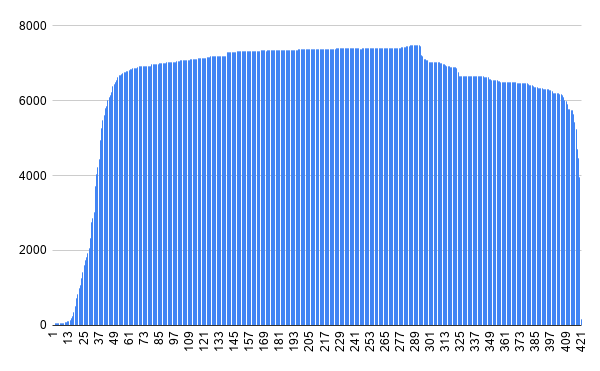
\includegraphics[width=\linewidth]{figures/position_coverage}
    \caption{Position coverage}
    \label{fig:positionCoverage}
\end{figure}

In this histogram, we can see that positions on the beginning have low coverage, and so
do few positions in the end. Because of this, we only took only those reads which cover all
positions between 50 and 408 (both included). As reads cover all positions from 50 to 408, there
is no longer a problem with unavailable information about modifications. Even though not all reads 
are taken into consideration for clustering, more than 50\% of them are.

Due to the error rate induced by sequencing, only those positions where at least 10\% of reads
had modification on were taken into consideration. The input for every read is a map where keys 
are only these positions and the values are 0 or 1 depending on if there was a modification on a 
certain position.

In the python sklearn library, there is the KMeans class which has, among other functions, a fit function.
This function takes as a parameter training instances to cluster in the form of an array-like, sparse matrix 
of shape (n\_samples, n\_features) and it returns a fitted estimator. Because of this, the data
is not given in the form of a list of maps, it was first transformed using sklearn's DictVectorizer
class and its function called fit\_transform on whose result the function toarray() was called \cite{dictVectorizer}.

\subsection{Determining the Optimal Number of Clusters}
The fundamental issue for the K-Means algorithm is determining the optimal 
number of clusters in a data set. There is no definite answer to this question and it 
depends on the method used for the determining. 
There are direct methods such as the elbow method and the silhouette method, and there are
also statistical testing methods, such as gap statistic. 

\subsubsection{Elbow Method}
As said before, the elbow method is a heuristic used for determining the optimal number of
clusters in a data set. The method consists of the following steps:
\begin{enumerate}
    \item Computing the K-Means algorithm for various values of k. 
    \item For each k, calculate the total within-cluster sum of squares
    (K-Means from sklearn library already has the attribute inertia which gives this number).
    \item Plotting the curve of the within-cluster sum of squares to the number of clusters k \cite{optimalKmethods}.
\end{enumerate}

\begin{figure}[H]
    \centering
    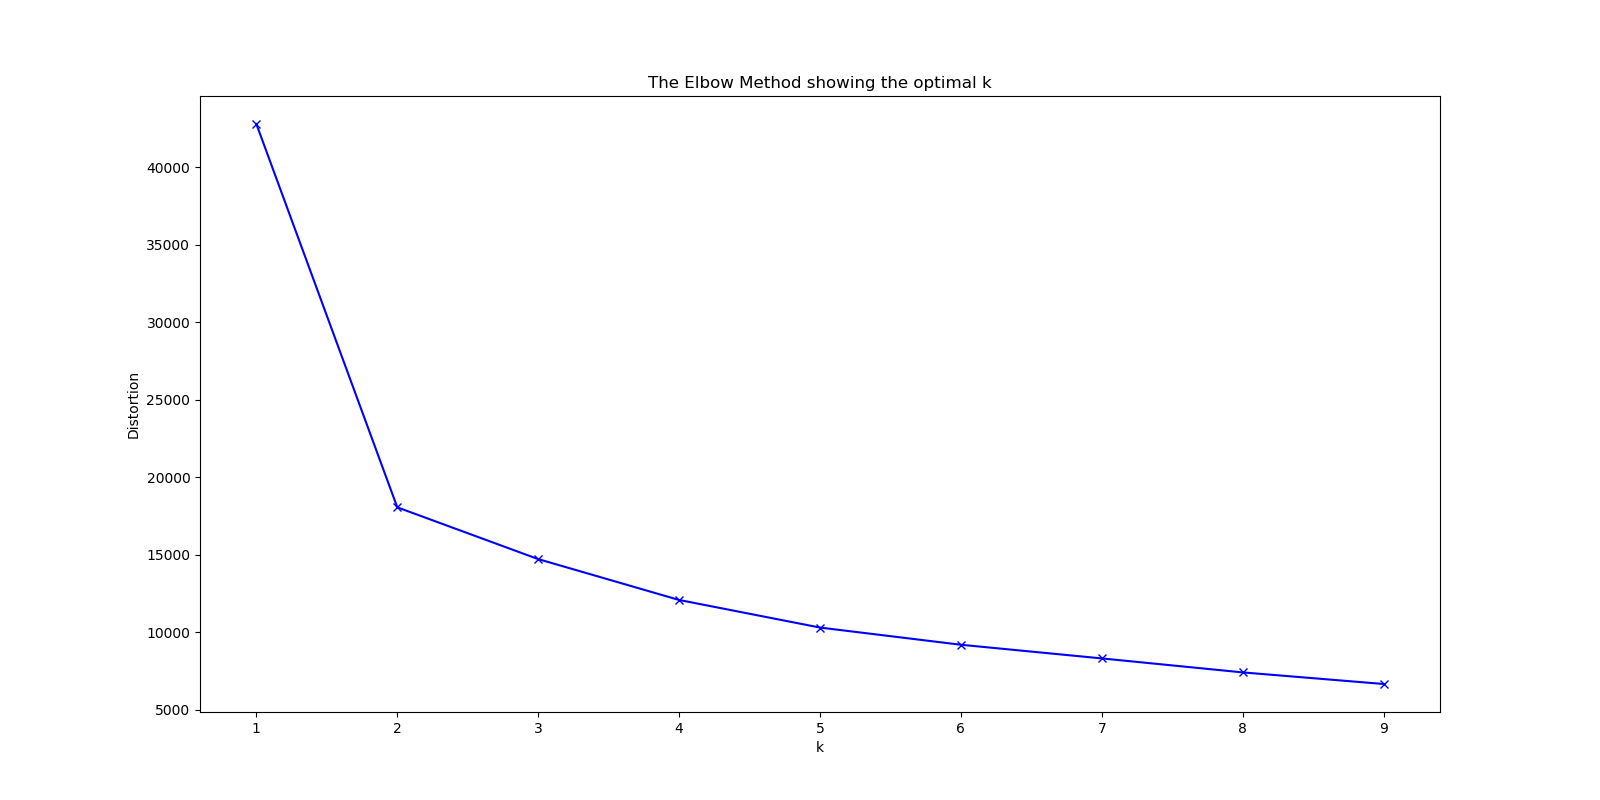
\includegraphics[width=\linewidth]{figures/elbow_method}
    \caption{Elbow method showing the optimal number of clusters}
    \label{fig:elbowMethod}
\end{figure}

The number of clusters to use in the K-Means algorithm is the value of parameter k where 
the elbow of the curve is. On figure \ref{fig:elbowMethod} we can see that k = 4 could be the optimal value.

\subsubsection{Silhouette Method}
The silhouette method provides a succinct graphical representation of how well each object has been classified.
The technique measures the similarity of an object to its cluster compared to other clusters \cite{optimalKmethods}.

The Silhouette Coefficient of a sample is equal to  $ \frac{b - a}{max(a, b)}$ where a represents
the mean intra-cluster distance and b represents the mean nearest-cluster distance.
In the sklearn library, there is a silhouette\_score function which returns the mean 
Silhouette Coefficient of all samples. There is also a function called silhouette\_samples 
which returns the Silhouette Coefficient for each sample \cite{silhouetteSamples}.

A visual representation of the silhouette method and clustered data using PCA is shown in figures
\ref{fig:silhouette1} to \ref{fig:silhouette6}. On the left side of every figure is a
representation of all the clusters and one horisontal line which represents the average 
silhouette score. On the right side is visual representation of clusters using the PCA 
algorithm.

\begin{figure}[H]
    \centering
    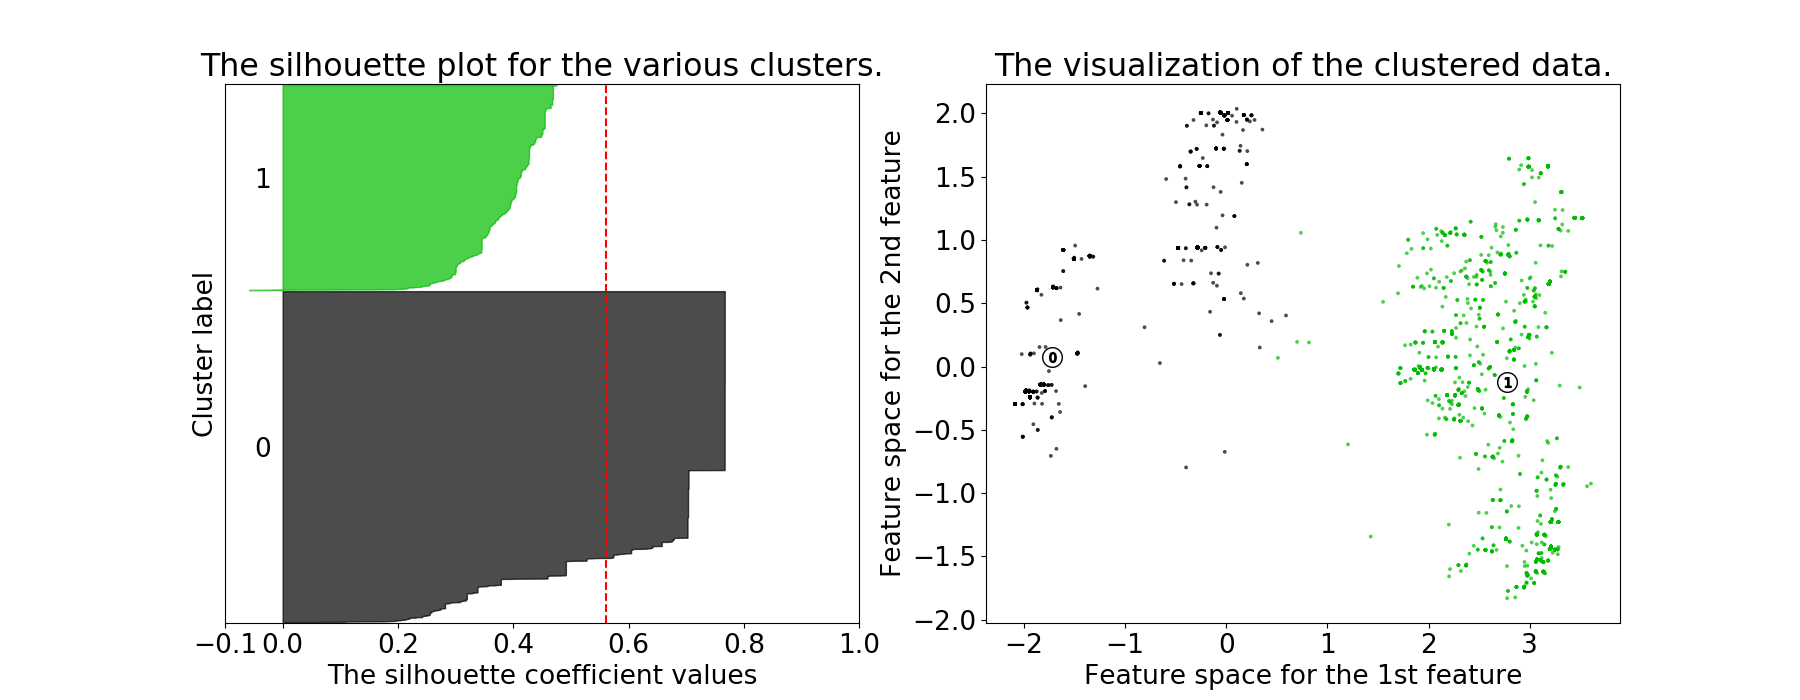
\includegraphics[width=\linewidth]{figures/silhouette_2}
    \caption{Silhouette scores and data visualization using PCA for k = 2}
    \label{fig:silhouette1}
  \end{figure}

  \begin{figure}[H]
    \centering
    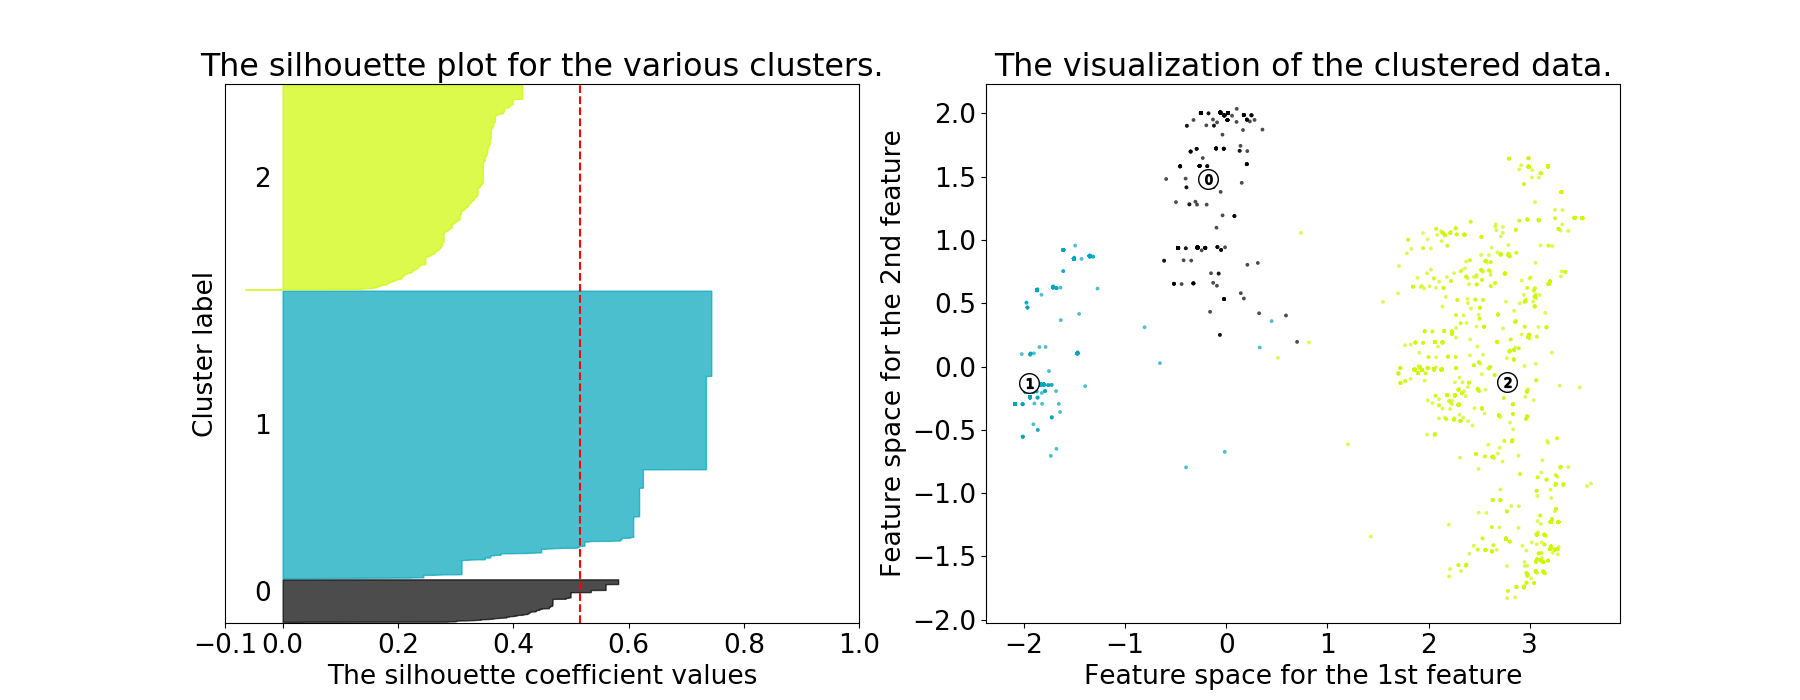
\includegraphics[width=\linewidth]{figures/silhouette_3}
    \caption{Silhouette scores and data visualization using PCA for k = 3}
    \label{fig:silhouette2}
  \end{figure}

  \begin{figure}[H]
    \centering
    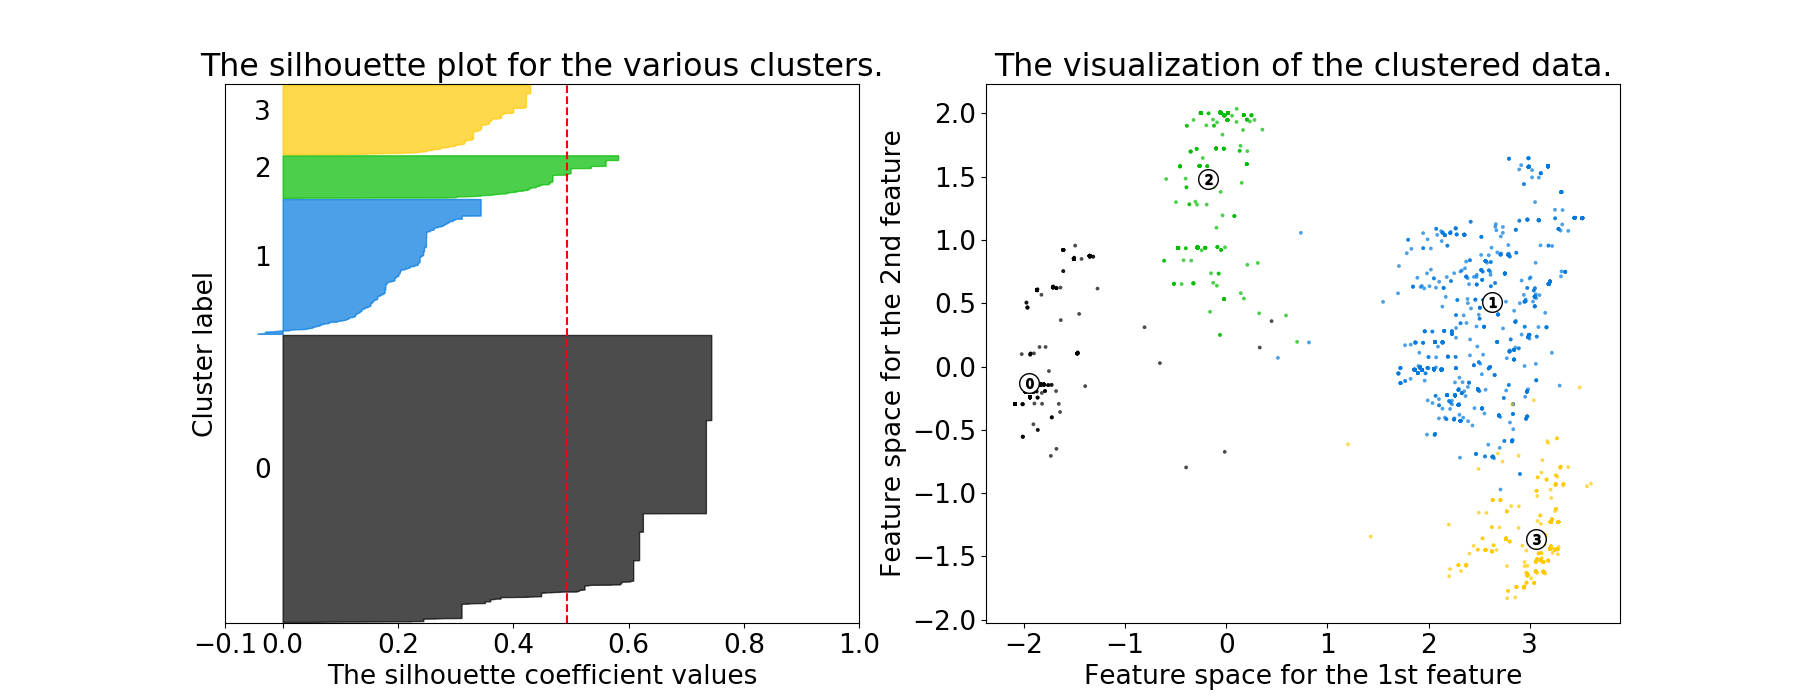
\includegraphics[width=\linewidth]{figures/silhouette_4}
    \caption{Silhouette scores and data visualization using PCA for k = 4}
    \label{fig:silhouette3}
  \end{figure}

  \begin{figure}[H]
    \centering
    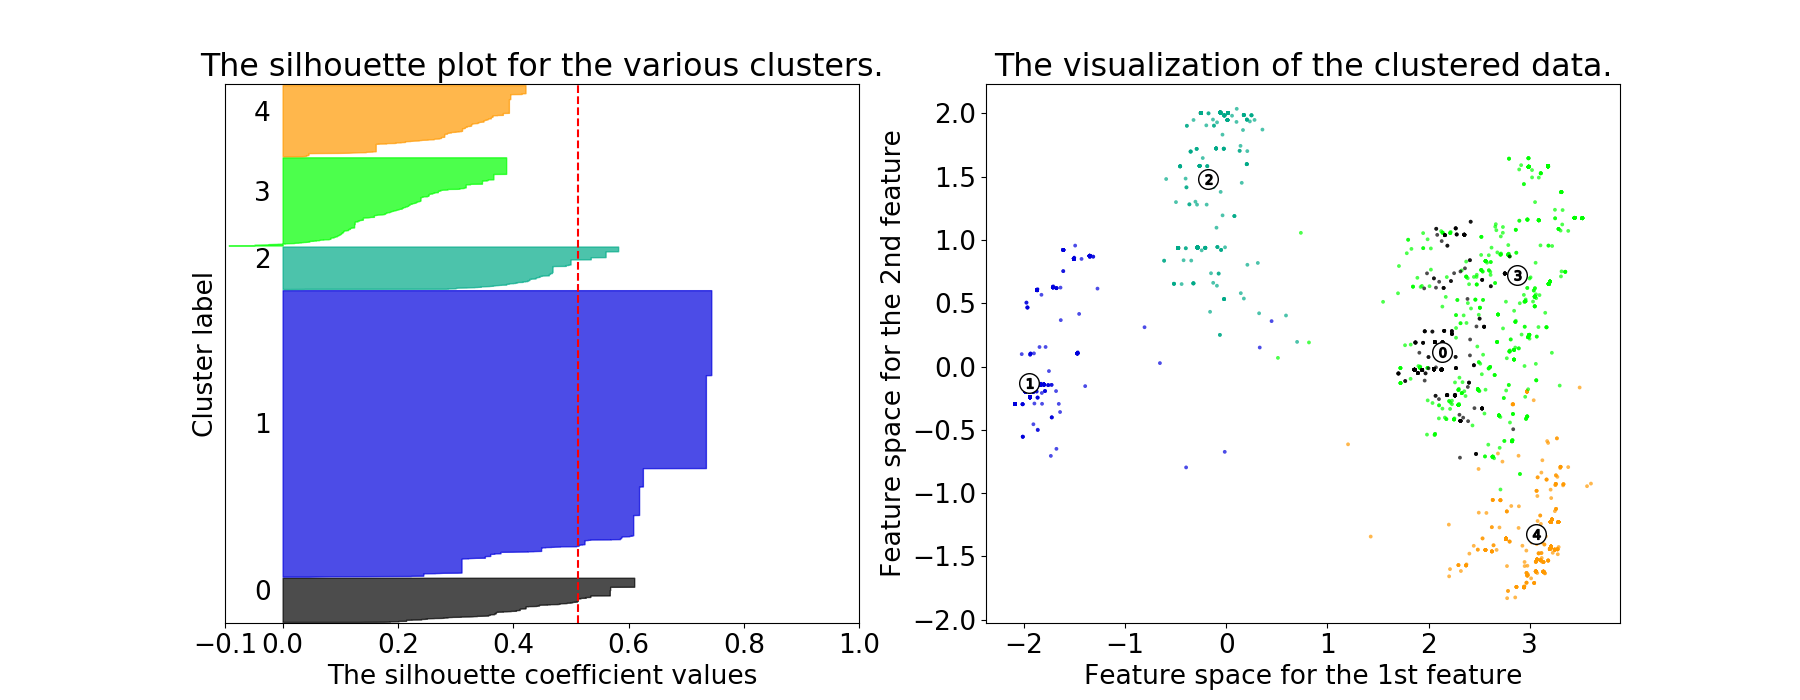
\includegraphics[width=\linewidth]{figures/silhouette_5}
    \caption{Silhouette scores and data visualization using PCA for k = 5}
    \label{fig:silhouette4}
  \end{figure}

  \begin{figure}[H]
    \centering
    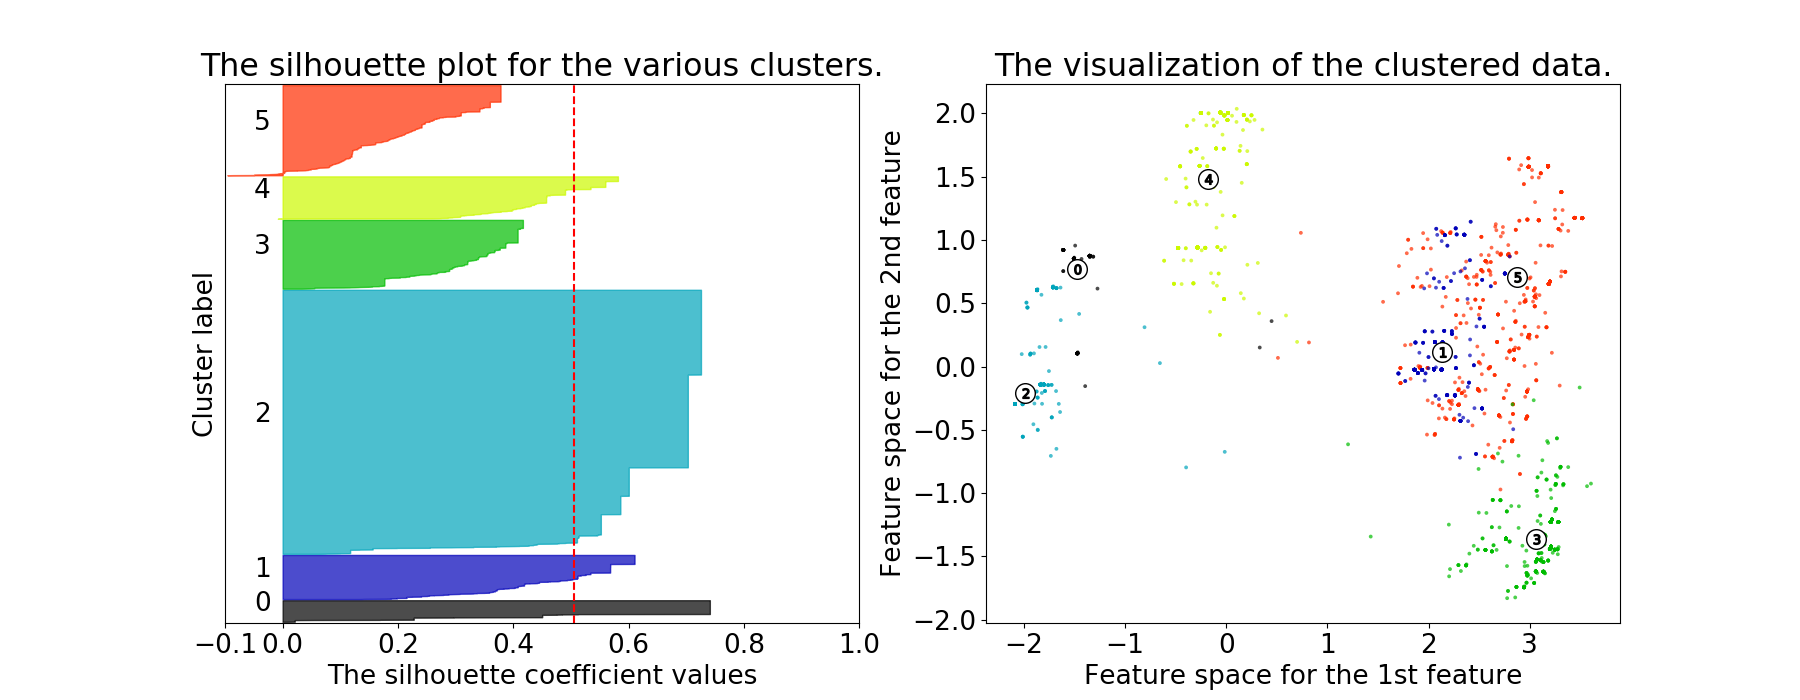
\includegraphics[width=\linewidth]{figures/silhouette_6}
    \caption{Silhouette scores and data visualization using PCA for k = 6}
    \label{fig:silhouette5}
  \end{figure}

  \begin{figure}[H]
    \centering
    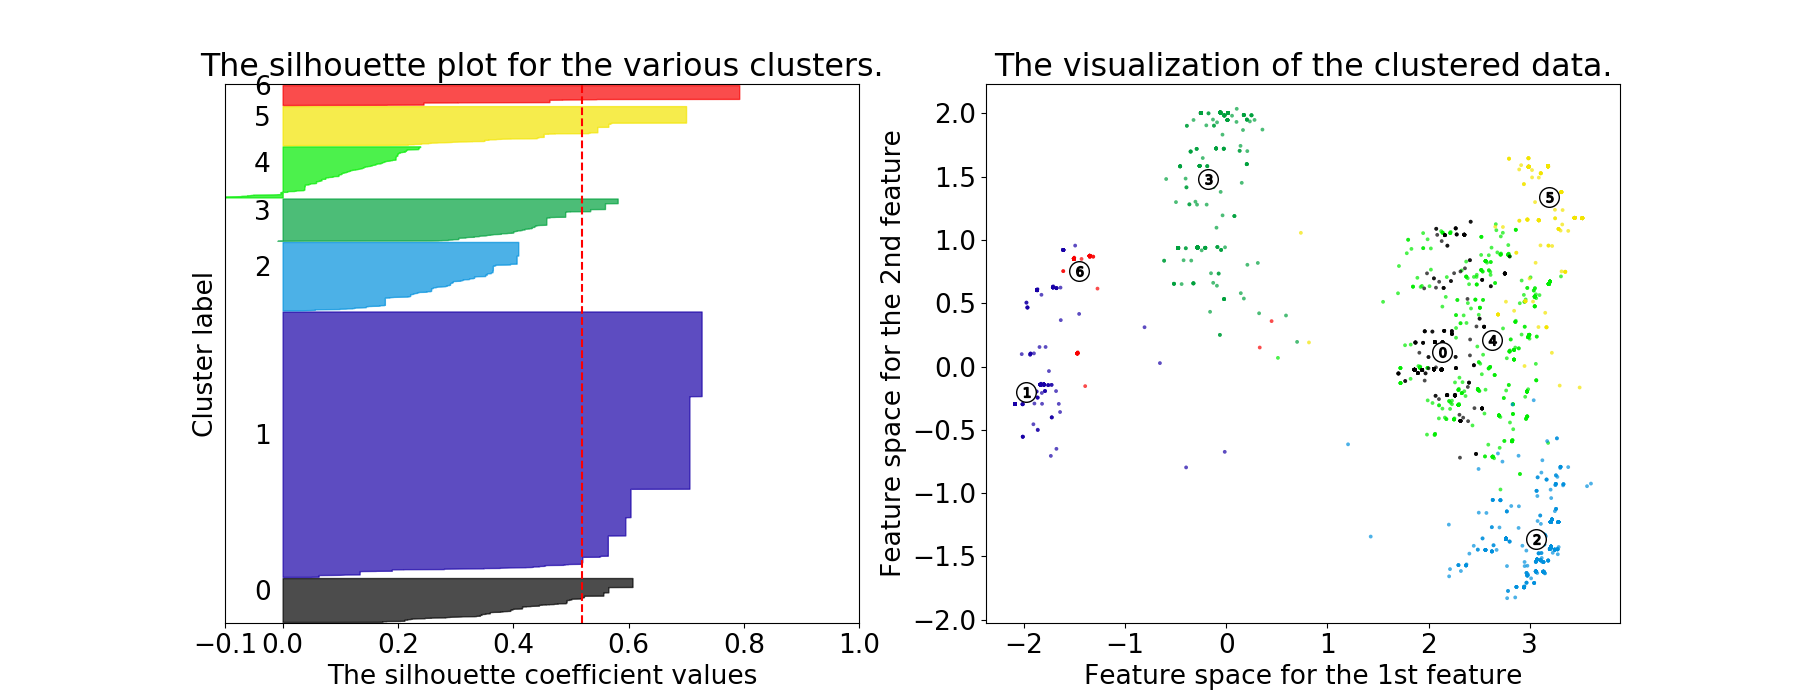
\includegraphics[width=\linewidth]{figures/silhouette_7}
    \caption{Silhouette scores and data visualization using PCA for k = 7}
    \label{fig:silhouette6}
  \end{figure}

Determining the optimal k parameter with the silhouette method is not 
precise, but two guidances should be that it is bad if there are
clusters with below average silhouette scores present and if there are 
wide fluctuations in the size of the silhouette plots \cite{silhouetteDet}. None of the 
figures satisfy these conditions, but we could say that results for 
k = 4 are better than for other values. 

Taking into account the results obtained by the elbow method and the silhouette method, 
we can conclude that the optimal value of the parameter k should be 4. 

\subsection{Visualization}
For visualizing the multidimensional data on a two-dimensional graph, dimensionality reduction 
is needed. This is a process of reducing  the number of random variables under consideration, 
by obtaining a set of principal variables. Some of the various methods for dimensionality 
reductions are: Principal Component Analysis (PCA), Linear Discriminant Analysis (LDA), 
and Generalized Discriminant Analysis (GDA).

It is important to realize that even though there are great advantages to dimensionality reduction, 
such as data compression which results in reduced storage space, reduced computation time and 
removing redundant features, there are also some disadvantages. Some of the disadvatages include: some amount of data loss, 
PCA tending to find linear correlations between variables which is sometimes undesirable, and
PCA failing in cases where the mean and covariance are not enough to define datasets.

\subsubsection{PCA}
PCA stands for Principal Component Analysis. This algorithm reduces dimensionality, 
increases interpretability but at the same time minimizes information loss. It creates 
new uncorrelated variables which maximize the variance and minimize the error. These new 
variables are called the principal components. Conceptually, the principal components
represent some amount of every one of the attributes. Finding these components is 
equal to solving an eigenvalue/eigenvector problem \cite{pca}.

\begin{figure}[H]
    \centering
    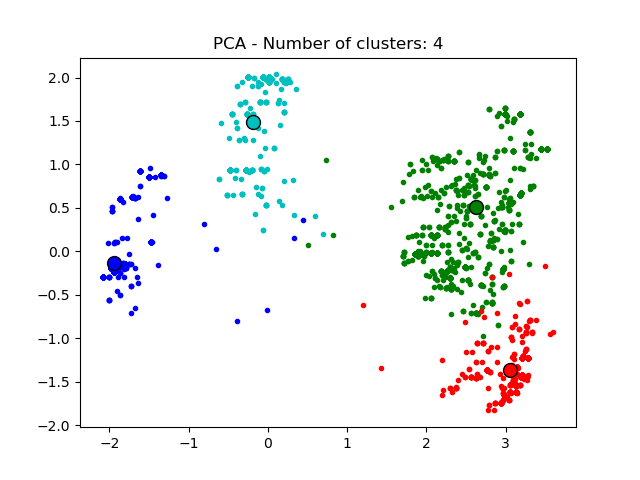
\includegraphics[width=\linewidth]{figures/4_clusters.png}
    \caption{KMeans with 4 clusters, PCA algorithm}
    \label{fig:4pca}
\end{figure}

Figure \ref{fig:4pca} shows a visual representation of clusters 
obtained by executing the K-Means algorithm. The figure was obtained
using sklearn's PCA class \cite{pcaSklearn}.

\subsubsection{t-SNE}
T-SNE stands for t-distributed Stochastic Neighbor Embedding. It is a machine learning
algorithm for reducing the high-dimensionality dataset into a low-dimensional space while 
retaining a lot of original information. The algorithm consists of two main 
stages. First, it constructs a probability distribution over pairs of high-dimensional 
objects in a way that the distribution is proportional to the similarities between objects
in the high dimensional space. In the second stage, t-SNE makes a similar
probability distribution in the low-dimension, this time using Student t-distribution, 
while trying to minimize the Kullback-Leibler divergence using the gradient descent. 
Because t-SNE has a non-convex cost function, different initializations can lead to a different result \cite{tsne}.

The visualization using t-SNE for results from the K-Means algorithm with k = 4 is shown on 
figures \ref{fig:tsne30} and \ref{fig:tsne45}. The results are volatile depending on the 
value of the parameter perplexity. They were obtained using sklearn's TSNE class \cite{tsneSklearn}.

\begin{figure}[H]
    \centering
    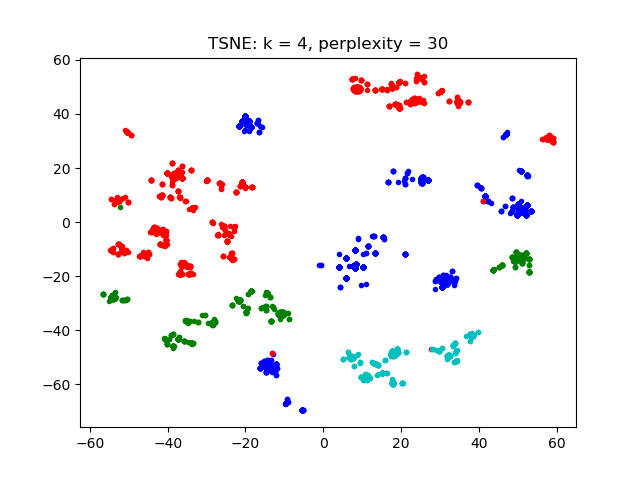
\includegraphics[width=\linewidth]{figures/tsne}
    \caption{KMeans with 4 clusters, t-SNE algorithm, default perplexity (30)}
    \label{fig:tsne30}
\end{figure}

\begin{figure}[H]
    \centering
    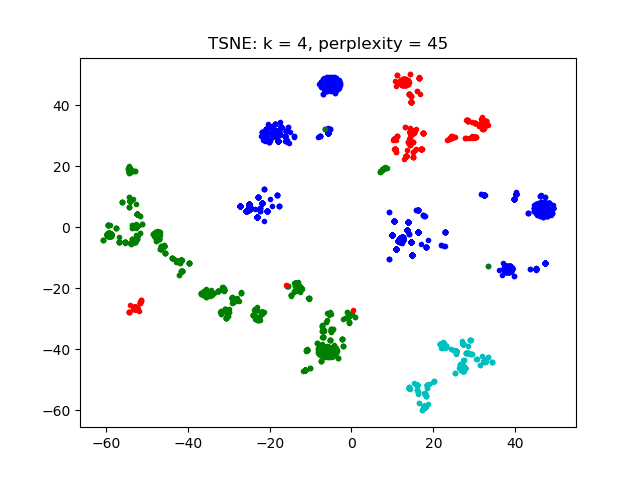
\includegraphics[width=\linewidth]{figures/tsne_perplexity45}
    \caption{KMeans with 4 clusters, t-SNE algorithm, perplexity 45}
    \label{fig:tsne45}
\end{figure}

In these figures, the clusters are not noticeable and this is the 
reason why the PCA algorithm is chosen for the pipeline. 

The main difference between t-SNE and PCA is that t-SNE preserves only small pairwise
distances or local similarities and PCA preserves large pairwise distances to maximize
variance. 

\chapter{Results}
This chapter is dedicated to showcasing results and performances. \\
In figure \ref{fig:tablet} on the top part we can notice red vertical stripes which 
represent modifications. There are some positions with modifications 
on almost all reads covering that position. On the bottom part of the figure, we can 
see part of the reads positioned as a horizontal red line on the part presents. In the 
middle, we can notice two nucleotides C instead of two nucleotides T. Also, on the left
and the right part of the figure, some deletions are shown. Looking at these deletions, 
it is clear that not all the reads have the same modifications, which indicates the 
existence of the clusters.

\begin{figure}[H]
    \centering
    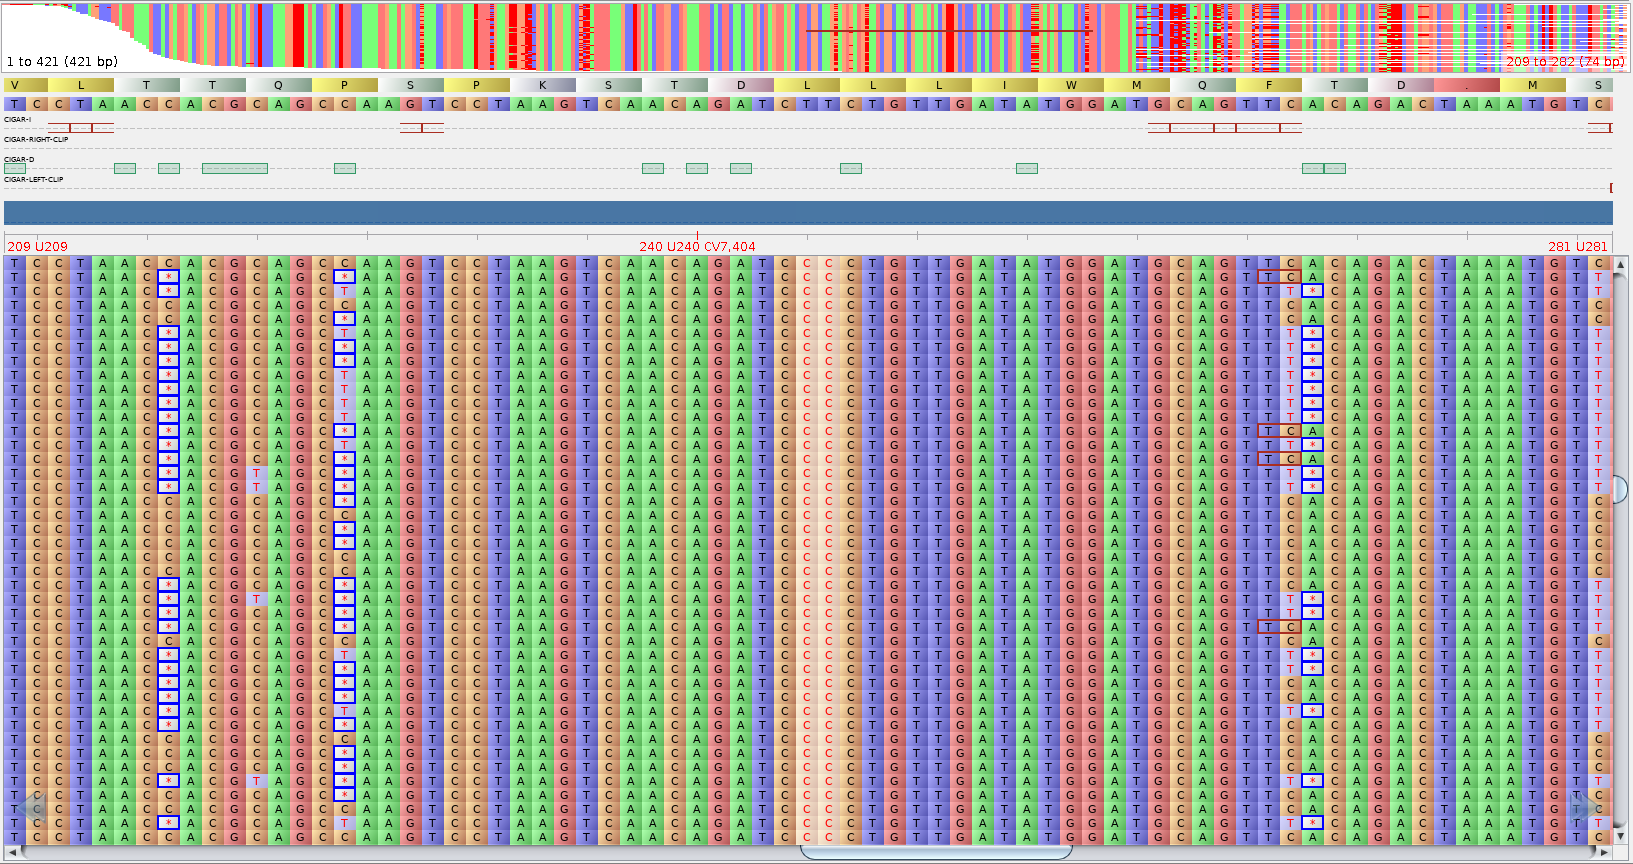
\includegraphics[width=\linewidth]{figures/tablet}
    \caption{Screenshot from Tablet \cite{tablet}}
    \label{fig:tablet}
\end{figure}

Figure \ref{fig:modFreq} shows the number of the modifications on every position. This graph
does not take into account which modification is on a certain position which means there 
could be deletion and mismatch on the same position and both would be counted as a modification
on that position.

\begin{figure}[H]
    \centering
    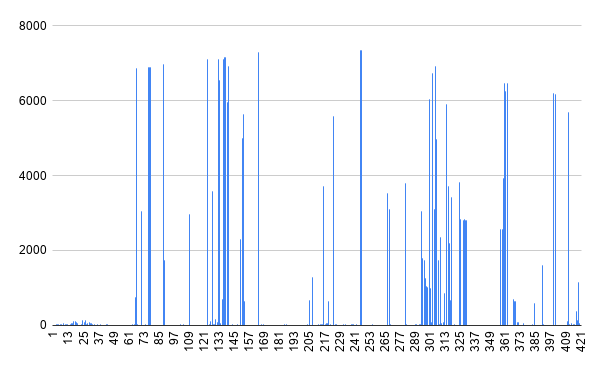
\includegraphics[width=\linewidth]{figures/modification_frequency}
    \caption{Modification frequency}
    \label{fig:modFreq}
\end{figure}

Some of the results were shown in the previous chapter as reviews of 
how the algorithms work. These results were obtained by implementing 
the read selection and polishing with Graphmap as the main tool.
This is once again a consequence of Dominik's work in Singapore, where
he decided that the best combination of parameters is given in this command:
\begin{lstlisting}[language=bash]
graphmap align --freq-percentile 1.0 --double-index 
--minimizer-window 1 -k 6 --ambiguity 0.5 
--auto-rebuild-index
\end{lstlisting}
This command was used in the read selection, for the final alignment and 
the version of this command where '-x overlap' was added
for creating the overlaps file for Racon in the polishing part.

The main disadvantage of this pipeline is its execution time. Using Racon 
for polishing and repeating polishing multiple times while creating overlaps
in between every polish creates a bottleneck. Polishing is the main reason 
why the number of reads that could be aligned to the reference is increased 
after this step, so polishing can not be removed from the pipeline.

In a previously mentioned implementation, another factor for longer execution time is
using Graphmap for overlaps. These two combined, make this pipeline unusable 
for data with a significant number of reads or with more transcripts in the
reference. Even for the given data with only 9951 reads and one pretty short 
reference, the results were not unavailable due to the pipeline taking too long. 
Because of this, reads were split into batches with 1000 reads or less and 
after the final alignment, results were combined in one and clustering was done 
afterwards. 

One of the main reasons why Ram was not selected as the main tool for the pipeline
was mapping a significant number of reads to other transcripts. 
This feature is undesirable when the reference consists of many transcripts. 
The reference for the research for this thesis has only one transcript, so 
this was not a problem. As a result, in the second implementation, Ram was 
used for alignment and overlapping. \\
It was not used for the final alignment as for now it can only produce output in a
paf format, and cigar string is needed in the process of clustering to determine 
if there was a modification on a certain position. Instead, Graphmap with 
default parameters was used, because it gave the best results of all 
tested combinations. 

This implementation gave different results than the first so the position 
coverage after read selection and polishing is shown in figure \ref{fig:posCoverageRam}.

\begin{figure}[H]
    \centering
    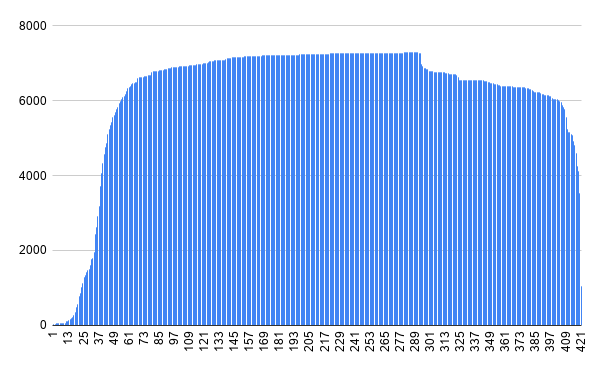
\includegraphics[width=\linewidth]{figures/ram_pos_coverage}
    \caption{Position coverage for the second implementation using Ram as the main tool}
    \label{fig:posCoverageRam}
\end{figure}

We can see that once again the beginning and the ending have low coverage, but it is
slightly better than in the previous case. 

The elbow method done with the data produced in the implementation with Ram confirmed 
that k = 4 is the optimal value for parameter k. 

\begin{figure}[H]
    \centering
    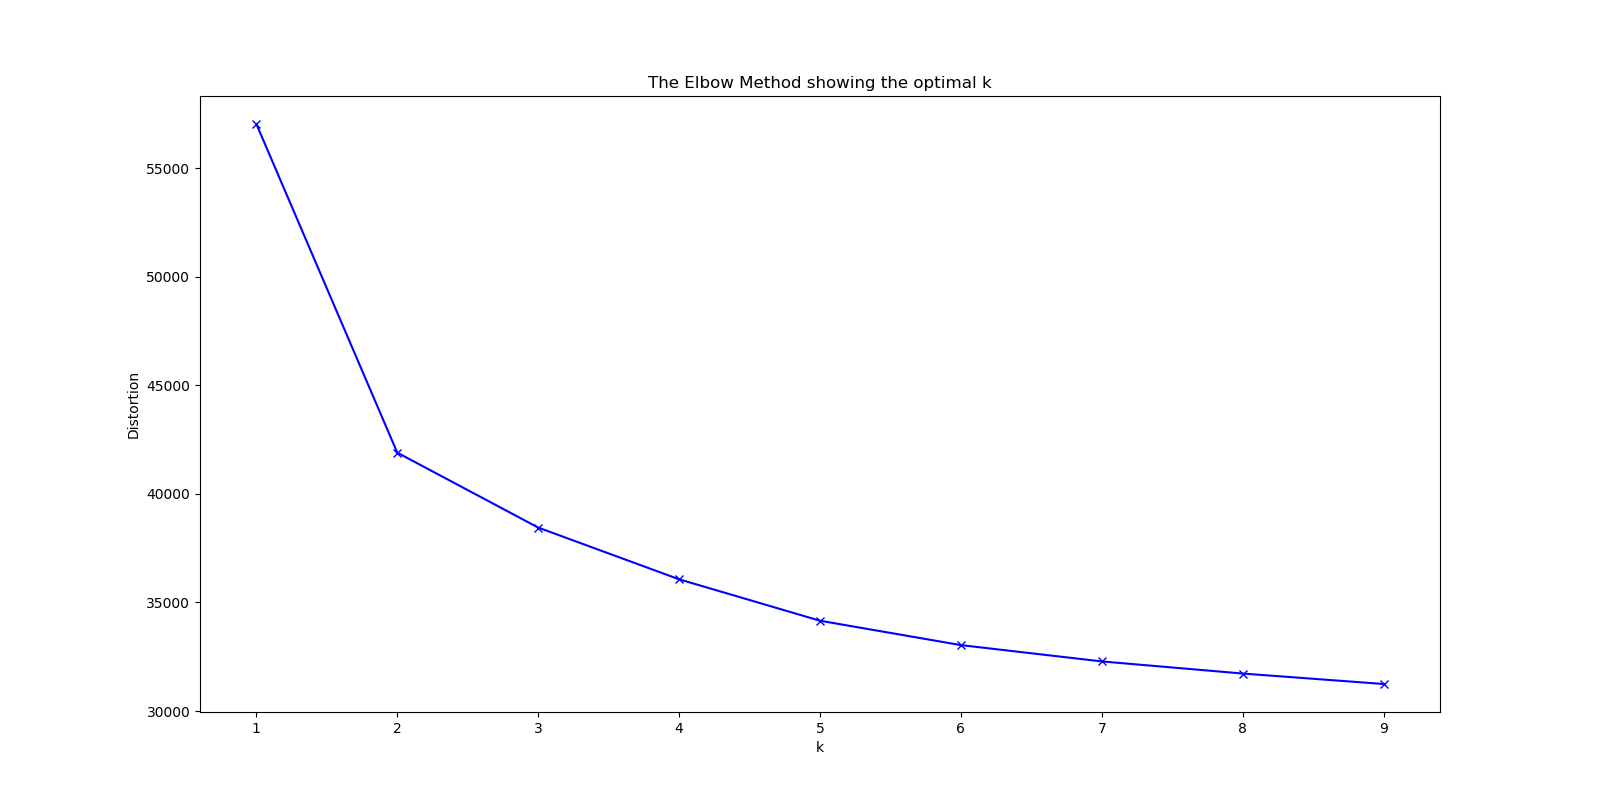
\includegraphics[width=\linewidth]{figures/elbow_process_ram}
    \caption{Elbow method with data from implementation using Ram}
    \label{fig:elbowRam}
\end{figure}

After read selection, there were 7638 reads of 9951 which successively mapped to 
the reference or to the mapped reads. Out of these 7638 reads, 4432 reads covered
all positions from 50 to 208 and those reads have been clustered. The result of 
clustering has been visualized using the PCA algorithm.

\begin{figure}[H]
    \centering
    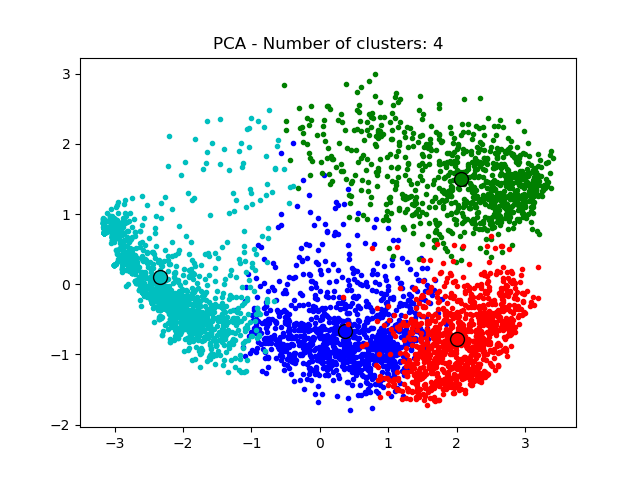
\includegraphics[width=\linewidth]{figures/ram_final_graphmap_PCA_4}
    \caption{Clustering the data using Ram as the main tool for the previous steps}
    \label{fig:clustersRam}
\end{figure}

Ram made it possible to execute the pipeline with all 5x modified reads at once,
not divided in parts. It took more than 3 hours which is not acceptable, 
but at least it finished, unlike with Graphmap. If the reads were split in 
smaller batches, it could be even better. 
% TODO : možda još nešto dodaj

\chapter{Conclusion}
The main concern of this thesis is the clustering of modified nucleotides. We 
succeeded in getting the clusters, but there could be many improvements. 
As for the clustering, there could have been more complex methods implemented, 
such as the Expectation–Maximization algorithm or a Recurrent neural network (RNN)
with an autoencoder. It would be much better if not only those reads that cover 
a certain part of the reference, but all those reads that successfully mapped 
to the reference with some version of 'unavailable' to mark those positions 
that the read does not cover. 

Another problem with this pipeline is the execution time. Ram boosted the
execution time, but it was still too long. As mentioned before, execution time
when Ram is the main tool for all reads is 3 hours 10 minutes and with Graphmap 
the execution was cancelled after 4 hours. To compare the execution times, 
both versions of the pipeline was executed with only 1000 reads. The execution time
with Ram was 1 minute 43 seconds and with Graphmap it was 8 minutes 27 seconds.
With improving the tools during time, there could be improvements with time too. 

The implementation could also be improved with splitting the data into 
smaller batches, but this can only be done with reads and not with the 
reference. 

Every one of the tested tools has its advantages and disadvantages, 
the "perfect" tool would not align reads to the transcripts where 
it does not belong, would have acceptable execution time and could 
align reads regardless of the error rate. 

\bibliography{literatura}
\bibliographystyle{plainnat}

\begin{sazetak}
The main concern of this thesis is the clustering of modified nucleotides in nanopore
sequenced RNA reads. The data for this thesis are reads and the reference from the 
tetrahymena ribozyme, a group I intron from \textit{Tetrahymena}. The goal was to 
integrate existing tools such as Graphmap, Minimap and Minimap2, Ram, and Racon
and link them with python scripts into a pipeline. To do this, all of the alignment 
tools were tested. A different approach for alignment was also tried out, aligning 
the reads in the signal domain. The pipeline was implemented in three parts: read
selection, polishing and clustering of modified nucleotides. 
Source code is available at: \url{https://github.com/lbcb-edu/BSc-thesis-19-20/tree/imartinovic}.

\keywords{RNA, pipeline, nanopores, modifications, sklearn, alignment}
\end{sazetak}

% TODO: Navedite naslov na engleskom jeziku.
\engtitle{Protočna struktura za detekciju grupa modificiranih nukleotida u očitanjima RNA dobivenih metodom nanopora}
\begin{abstract}
Glavna zadaća ovog rada je detekcija grupa modificiranih nukletida u očitanjima 
RNA dobivenih metodom nanopora. Podaci za ovaj rad su očitanja i referenca ribozima 
tetrahimena, skupine I introna iz \textit{Tetrahymena}. Cilj je bio integirati 
postojeće alate kao što su Graphmap, Minimap i Minimap2, Ram, i Racon te ih povezati
python skriptama u protočnu strukturu. Kako bi se to napravilo, svi alati za 
poravnavanje bili su testirani. Drugačiji pristup je također proban, poravnavanje
očitanja u domeni signala. Protočna struktura sastoji se od tri dijela: odabira 
očitanja, poliranja i detekcije grupa modificiranih nukleotida.
Izvorni kod dostupan je na: \url{https://github.com/lbcb-edu/BSc-thesis-19-20/tree/imartinovic}.

\kljucnerijeci{RNA, protočna struktura, nanopore, modifikacije, sklearn, poravnavanje}
\end{abstract}

\end{document}
